\subsection{Aus einer Menge $N$ mit $n$ Elementen sollen alle oder $k$ Elemente ausgewählt werden}

\begin{figure}[h]
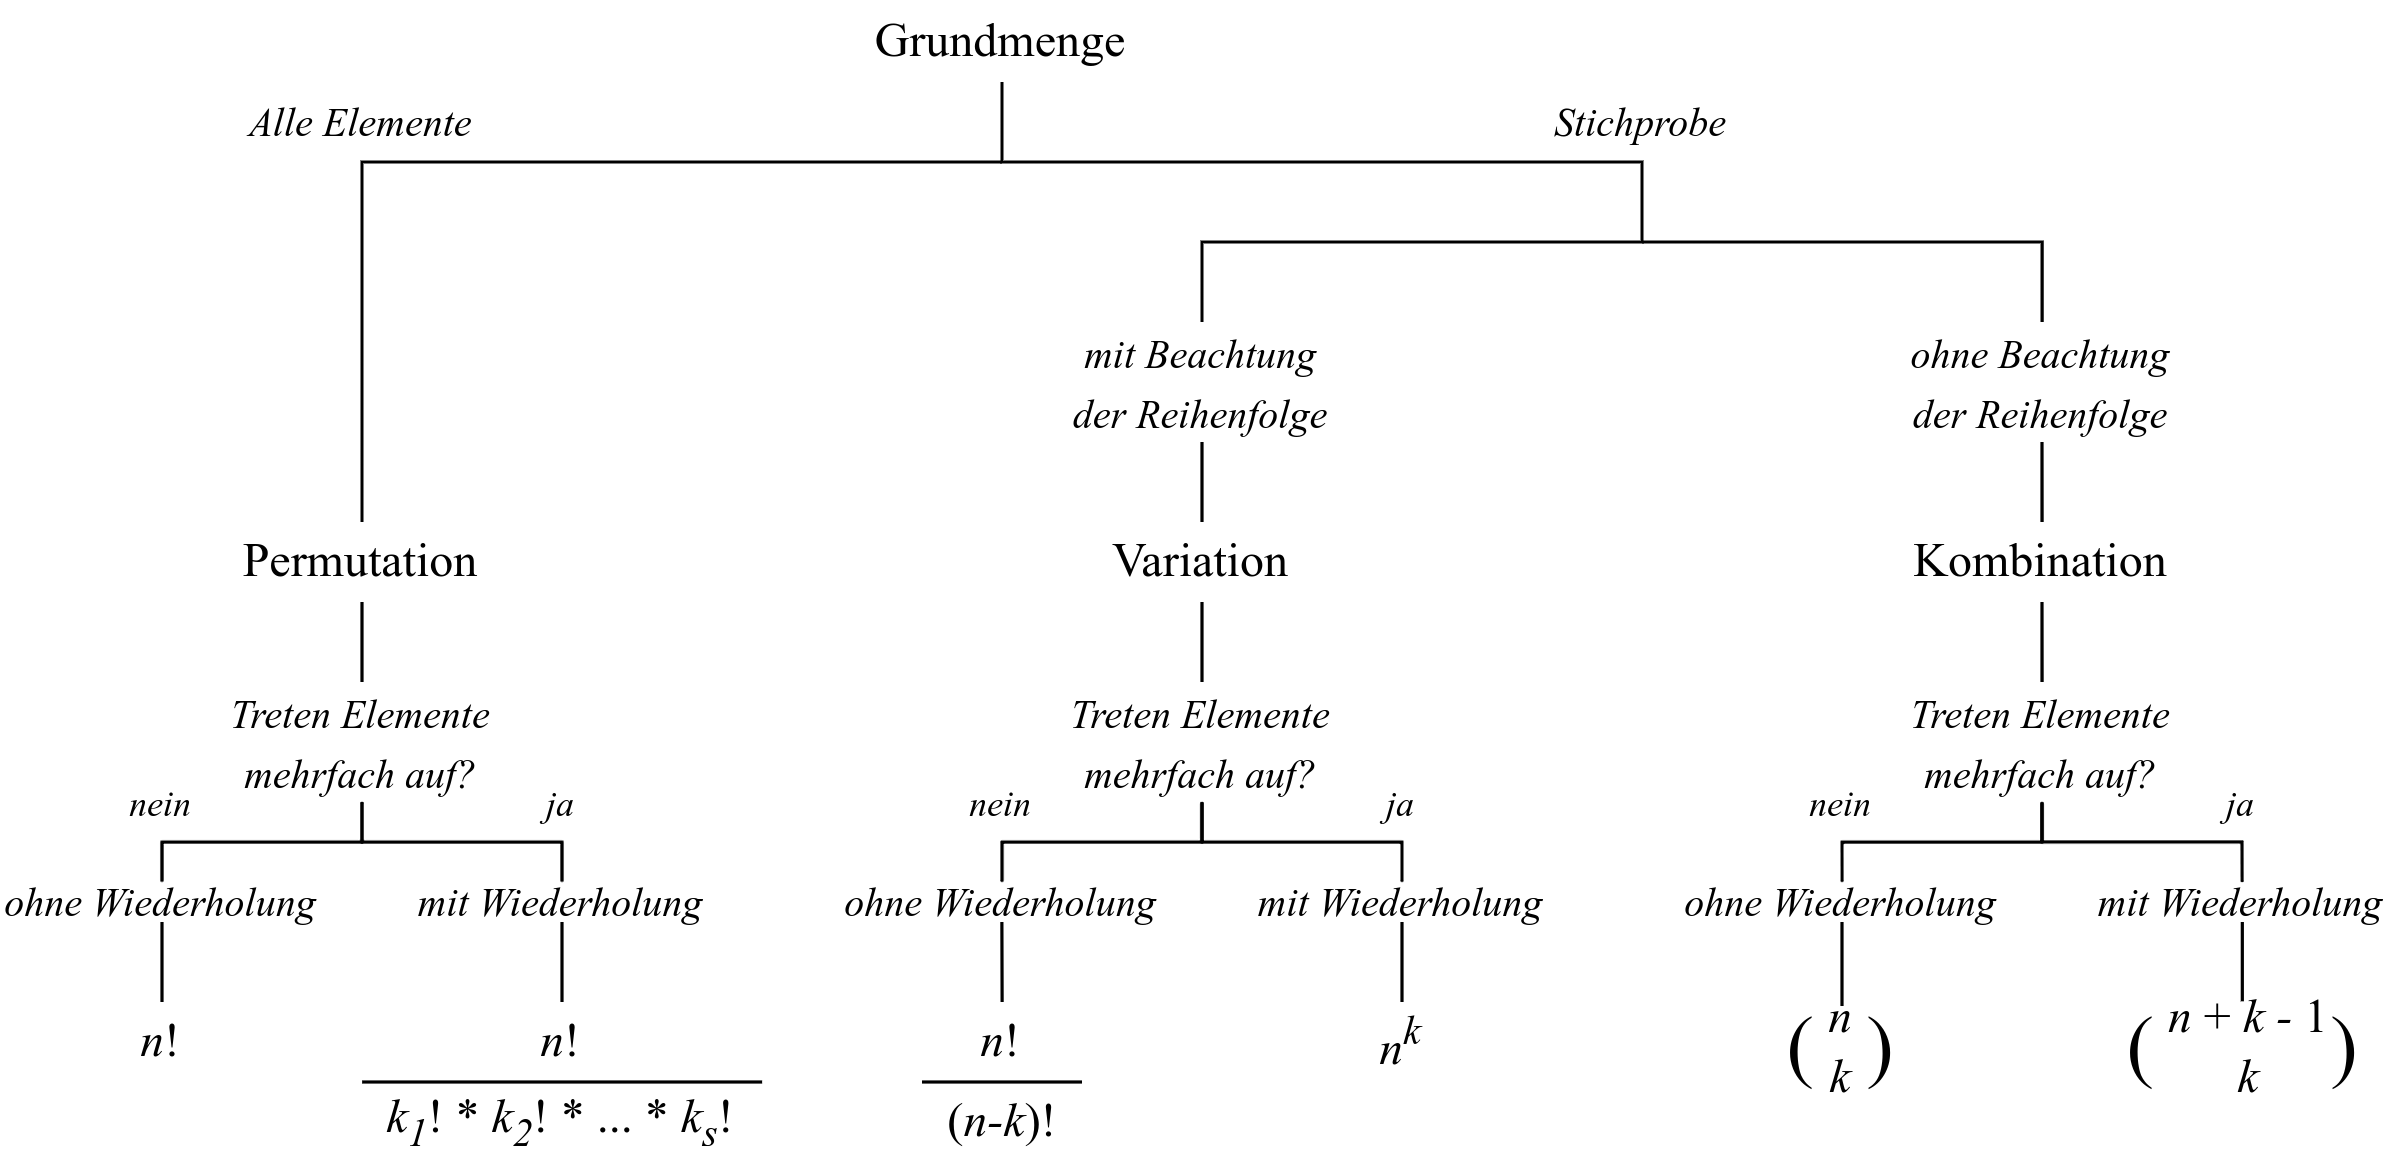
\includegraphics[width=1\textwidth]{graphics/komb_baum.png}
\end{figure}

{
\footnotesize
\begin{itemize}[leftmargin=*]
\item \textit{Mit Beachtung der Reihenfolge:} ABC $\not =$ ACB $\not =$ BAC $\not =$ BCA $\not =$ CAB $\not =$ CBA
\item \textit{Ohne Beachtung der Reihenfolge:} ABC $=$ ACB $=$ BAC $=$ BCA $=$ CAB $=$ CBA
\end{itemize}
}

\subsubsection*{Kombination:}

\textbf{Exakte Auswahl:} Aus einer Menge mit $n$ Elementen wählt man (\textit{genau}) $k$ aus.

$$
\begin{pmatrix}
n\\
k
\end{pmatrix} =
\frac{n^{\underline{k}}}{k!}
$$

\textbf{Mindestauswahl (Allgemein):} Wie viele Möglichkeiten gibt es \textit{mindestens} k von n (z.B mindestens 7 von 10) richtig zu beantworten?

\begin{itemize}[leftmargin=*]
\item Man rechet immer mit Plus ($+$)
\end{itemize}

$$
\begin{pmatrix}10\\7\end{pmatrix} + \begin{pmatrix}10\\8\end{pmatrix} + \begin{pmatrix}10\\9\end{pmatrix} + \begin{pmatrix}10\\10\end{pmatrix} = 176
$$

\textbf{Mindestauswahl (mit getrennter Betrachtung):} Wie viele Möglichkeiten gibt es, falls von den ersten 5 Fragen \textit{genau} 3 und von den nächsten 5 \textit{genau} 4 richtig beantwortet werden müssen?

\begin{itemize}[leftmargin=*]
\item Man rechet immer mit Mal ($\cdot$)
\end{itemize}

$$
\begin{pmatrix}5\\3\end{pmatrix} \cdot \begin{pmatrix}5\\4\end{pmatrix} = 50
$$

\textbf{Mindestauswahl (mit kombinierter Betrachtung):} Wie viele Möglichkeiten gibt es, falls von den ersten 5 Fragen \textit{mindestens} 3 richtig beantwortet und insgesamt \textit{genau} 7 richtig beantwortet werden müssen?

\begin{itemize}[leftmargin=*]
\item Man rechet immer mit Plus ($+$) und Mal ($\cdot$)
\end{itemize}


$$
\begin{pmatrix}5\\3\end{pmatrix} \cdot \begin{pmatrix}5\\4\end{pmatrix} + \begin{pmatrix}5\\4\end{pmatrix} \cdot \begin{pmatrix}5\\3\end{pmatrix} +
\begin{pmatrix}5\\5\end{pmatrix} \cdot \begin{pmatrix}5\\2\end{pmatrix}
$$